\section{L3 Cache Size Sensitivity}
\label{sec:results:l3size_sensitivity}


\begin{figure}[th]
    \centering
    \includegraphics[scale=0.7]{figures/results/speedup/l3-stp-04M-all-l3}
    \caption[Speedup wtih decreasing L3 size]{Speedup of cache partition algorithms normalized to LRU with decreasing shared L3 size}
    \label{fig:results:l3}
\end{figure}

In this section, we cover an experiment where we run all 4-core workloads with varying L3 cache size.
While we have already shown in Section~\ref{sec:methodology:processor_model} that our simulated model is realistic compared to current processor architectures, we want to explore how algorithm performance changes when we constrain available L3 cache.
This experiment uses the same simulated system as in the cache partitioning experiment, Section~\ref{sec:results:cache_partition}.
We use four different L3 sizes; 4MB, 2MB, 1MB, and 0.5MB.
When we reduce the size of the shared cache level, we keep the associativity constant.
As a result, we have fewer sets in the cache and hence, more addresses map to the same set.
Table~\ref{tbl:processor_model:l3} shows detailed information about the two larger configurations.
The details for the two smaller configurations are equal to the L2 configurations of the same size, shown in Table~\ref{tbl:processor_model:l2}, but with an associativity of 32.
Fewer sets cause increased pressure on each set.
We expect to see some of the algorithms further their improvement over LRU in this situation.
Also, we expect PIPP, which already has shown bad performance compared to LRU, to continue this trend.

Before showing the results of this experiment, we will briefly discuss a special case that arises in this experiment.
When we set the L3 cache to 0.5MB, we have a situation where the sum of the L2 caches equals the L3 cache.
In this situation, with inclusive caches, it might be reasonable to think that no algorithm will outperform LRU.
As we will demonstrate, this is not the case.
In a simplified situation with two core, core 0 has a streaming access pattern and core 1 has a recency friendly pattern that fits in the L2 cache.
The L3 size is equal to the sum of L2s, and all caches are managed by LRU.
Consider the situation when core 0 has filled its L2 cache and core 1 has all its data in the private caches.
When execution continues core 0 to load new data, evicting old data from the L2 cache.
The data evicted will still be present in the L3 cache, inclusive caches only require that the data present in one cache level must be present in all lower levels.
Core 1 will never access the L3 cache because all data is present in the private caches. 
Hence the L3 cache blocks owned by core 1 will start to age, and they will eventually be evicted to fit new data loaded by core 0.
When this happens, the blocks are also evicted from core 1's private caches, to perserve the inclusive property.
Core 1 will start to miss, and will have to access main memory.
A perfect replacement scheme would shield core 1's blocks in the L3, causing an increase in performance for that core while not affecting the streaming core.
Because of this we conclude that a 0.5MB cache is valid, and we might observe an improvement over LRU.

Figure~\ref{fig:results:l3} show the speedup of all algorithms normalized to LRU for varying shared cache size.
DRRIP is the algorithm that shows least variation across the various shared cache sizes.
The figure shows DRRIP performing comparable to LRU in all cases, with a negligible increase of 0.3\% in the 1MB case.
TADIP that in the baseline scenario performs as good as LRU seems to suffer from the increased set pressure, with increasingly worse performance as the cache size decreases.
In our implementation, we scale the number of duel-sets relative to the total number of cache sets.
Hence, for both DRRIP and TADIP the fraction of duel sets is constant across the various L3 configurations.

As expected the performance of PIPP decreases as the set pressure increases.
We have previously, in Section~\ref{sec:results:cache_partition}, postulated that the potentially short lifetime of blocks in a PIPP managed cache may be the cause of the performance decrease compared to LRU.
This experiment further shows that when the number of accesses to a single set increases the performance of PIPP further decreases compared to LRU.
The MPKI in the 0.5MB cases, not shown here, is over 50\% worse than the LRU case, compared to only 20\% worse in the 4MB case.
PIPP-min8, a modified version of PIPP, have previously been shown to improve performance over normal PIPP replacement.
This is also the case when reducing shared cache size.
Figure~\ref{fig:results:l3} shows that PIPP-min8 not only performs as good as LRU in the base experiment, but with increased set pressure actually performs better than LRU.
With a 0.5MB L3 cache, the modified PIPP algorithm performs 4\% better than LRU measured in STP.
In the same configuration, the unmodified algorithm performs about 18\% worse compared to LRU.
This result clearly shows the advantage of the extended block lifetime in the modified PIPP algorithm, and at the same time points a fundamental performance problem with PIPP.


\begin{figure}[th]
    \centering
    \begin{subfigure}[b]{0.5\textwidth}
        \centering
        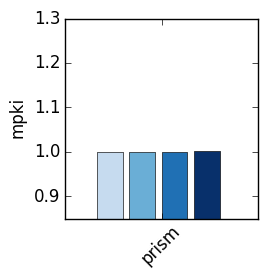
\includegraphics[width=0.8\textwidth]{figures/results/speedup/l3-mpki-04M-prism-l3}
        \caption{PriSM}
        \label{fig:results:l3:mpki-prism}
    \end{subfigure}%
    \begin{subfigure}[b]{0.5\textwidth}
        \centering
        \includegraphics[width=0.8\textwidth]{figures/results/speedup/l3-mpki-04M-ucp-l3}
        \caption{UCP}
        \label{fig:results:l3:mpki-ucp}
    \end{subfigure}
    \label{fig:results:l3:mpki}
    \caption{MPKI normalized to LRU with decreasing L3 cache size.}
\end{figure}

Next, we have PriSM, which shows a slight performance increase with the 2MB and 1MB cache. 
At both 4MB and 0.5MB PriSM performs as good as LRU.
Figure~\ref{fig:results:l3:mpki-prism} shows the MPKI for PriSM.
From this figure, we observe that PriSM in all configurations causes the same number of misses as LRU.
This is true even when PriSM shows an performance increase measured in STP.
Finally, we observe a performance increase by UCP in Figure~\ref{fig:results:l3}. 
In previous sections (\ref{sec:results:cache_partition} and \ref{sec:results:l2size_sensitivity}) we have shown that UCP is the top performer of our algorithms when measured in STP.
This is also the case in this experiment.
We observe that UCP increases performance compared to LRU in both the 2MB and 1MB case, in the 0.5MB case is comparable to the 1MB case.
Interestingly, Figure~\ref{fig:results:l3:mpki-ucp} shows that while UCP increases performance compared to LRU it also causes more misses, shown by an increase in MPKI.
Previous experiments have also shown this effect, as seen in Section~\ref{sec:results:cache_partition}.
